\documentclass{article}
\usepackage[utf8]{inputenc}
\title{Verification : TD4}
\author{Marius }
\date{October 2021}

\usepackage{stmaryrd}	%N
\usepackage{esvect}		%Vector
\usepackage{hyperref}	%hypertext link
\usepackage{graphicx}
\usepackage{amsmath}    %overset
\usepackage{amssymb}    %square
\usepackage{amsthm}		%proof
\usepackage{xcolor}		%color
\usepackage{esvect}		%Vector
\usepackage{tikz}		%draw
\usetikzlibrary{positioning}
\usetikzlibrary{automata}
\usetikzlibrary{arrows}



\newcommand{\V}{\mathcal{V}}
\newcommand{\A}{\mathcal{A}}
\newcommand{\N}{\mathbb{N}}
\newcommand{\R}{\mathcal{R}}
\newcommand{\T}{\mathcal{T}}

\begin{document}
\maketitle
\section*{Exercice 1}

Let $\A = (Q,\Sigma,I,T,(F_i)_{i\in\N})$. \newline
We build $(\A_i)_{i \in \N}$ such that $\A_i=(Q,\Sigma,I,T,F_i)$.\newline
Then we merge them by $T'(f_i,\alpha)=T(f_i,\alpha)_{i+1}$ \newline


\section*{Exercice 2}

$\bullet~Rat(\Sigma^\omega) \subseteq Rec(\Sigma^\omega)$\newline
Let $(X_i)_{i \leq m} \in Rat(\Sigma^*)$ and $(Y_i)_{i \leq m} \in Rat(\Sigma^+)$ and $(A_{X_i}, A_{Y_i})$ their automata.
Then $\underset{i\leq m}{\sum} (A_{X_i}.A_{Y_i}^\omega)$ recognize $\underset{i\leq m}{\bigcup} (X_i.Y_i^\omega)$ .\newline
$\bullet~Rec(\Sigma^\omega) \subseteq Rat(\Sigma^\omega)$\newline
$X_f=L(\A_f)$ vu comme un automate fini. $Y= \bigcup L(\A_{ff})$, où les $\A_{ff}$ sont des copies de $\A$ dont l'état initial est $f$. \newline
\color{olive} $\A_{ff}$ admet un état $f'$ copie de $f$ pour éviter d'accepter le mot vide.
\color{black}

\section*{Exercice 3}
\subsection*{a)}
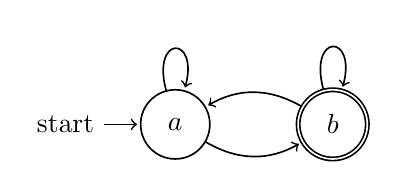
\begin{tikzpicture}[->,shorten >=1pt,auto,node distance=2cm,semithick]
\node[initial,state] (A)                    {$a$};
\node[accepting,state]         (B) [right of=A] {$b$};

\path (A)   edge[loop above]  node {} (A)
	  (A)   edge[bend right]  node {} (B)
      (B)   edge[bend right]  node {} (A)
      (B)   edge[loop above]  node {} (B);
\end{tikzpicture}
\subsection*{b)}

Let $\A$ be such an automata and $f_0 \in F$ reachable from $q_0$ by a word $u_0$.
Then, because $\A$ is deterministic and $u_0ba^\omega \in L$, there exists $u_1=bv_1$ such that $T^*(q_0,u_0u_1) \in F$.\newline
By induction, we may then build an infinite word $\underset{i \in \N}{\cdot}u_i$ containing an infinite number of $b$ and recognized by $\A$.
In particular, $L(\A) \neq L$

\subsection*{c)}

$L$ may be rewritten $\bigcup X.Y^*$ with the same construction as above. In that case $L' = \bigcup X.Y^\omega$\newline
Then $w$ has infinitely many prefixes if and only if $w \in \L'$, that is $L'=\vv{L}$


\section*{Exercice 4}




\newpage


\end{document}
